% !TEX root = ../ITGO.tex

\subsection*{Pressure vessel design problem}

In the pressure vessel design problem, the objective is to minimize the total manufacturing cost, including the cost of the material, forming and welding costs \citep{PV}. The problem is subject to three linear and one nonlinear inequality constraint, and its structure is shown in Figure \ref{fig:PV}. The four variables are the thickness of the shell ($x_1 = T_s$), the thickness of the head ($x_2 = T_h$), the inner radius ($x_3 = R$), and the length of the cylindrical section of the vessel ($x_4 = L$). This is an example of a mixed integer problem, where the first and second variables are constrained to be integers. The value of the objective function at the best known feasible solution is around $f(\bm{x}^*) = 6059.7143$.

\begin{figure}[h]
    \begin{center}
    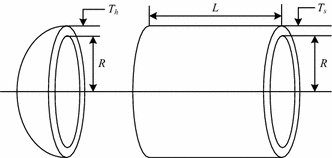
\includegraphics[scale=0.6]{Imgs/PV.png}
    \end{center}
    \captionsetup{justification=centering}
    \caption{Schematic view of pressure vessel design problem.}\label{fig:PV}
\end{figure}

\prob{Appendix/Problems/PV}